\section{Tính giá trị vout của tải $\mathbf{R_L}$ với transistor C2222A. Mô phỏng lại bằng proteus.}
    \subsection{Hình thứ nhất}
        \begin{figure}[H]
            \centering
            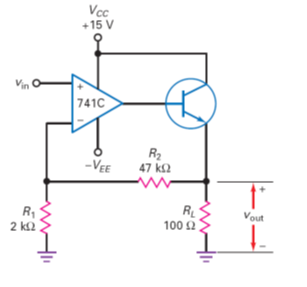
\includegraphics[width=0.7\textwidth]{pictures/topic4_a.png}
            \caption{Đề bài bài 4 hình thứ nhất}
        \end{figure}
        \subsubsection{Tính giá trị $V_{out}$ của tải $R_L$}
            \begin{itemize}
                \item Op-amp này nhận điện áp vào $V_{in}$ và khuếch đại. Tuy nhiên, điện áp ở đầu ra của op-amp không thể vượt quá nguồn cung cấp +15V và -15V.
                \item Transistor sẽ hạ hạ điện áp xuống một lượng $V_{BE} \approx 0.7V$ (giữa B và E) 
            \end{itemize}
            $\Rightarrow V_{out} = 15 - V_{BE} = 15 - 0.7 = 14.3V$.
        \subsubsection{Mô phỏng bằng proteus}
            \begin{itemize}
                \item Sử dụng Proteus để mô phỏng mạch như đề bài
                \item Các linh kiện sử dụng: Opamp, Resistor, Transistor, Voltage Source, Ground.
                \item Kết quả mô phỏng proteus.
                \begin{figure}[H]
                    \centering
                    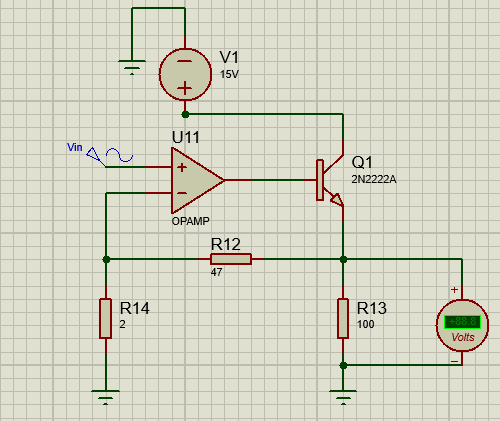
\includegraphics[width=0.7\textwidth]{pictures/result4_a.png}
                    \caption{Kết quả mô phỏng proteus bài 4 hình thứ nhất}
                \end{figure}
            \end{itemize}
            \hspace*{0.6cm}Từ kết quả mô phỏng proteus, ta thấy giá trị $V_{out}$ của tải $R_L$ là 14.3V, giống với kết quả tính toán.
    \subsection{Hình thứ hai}
        \begin{figure}[H]
            \centering
            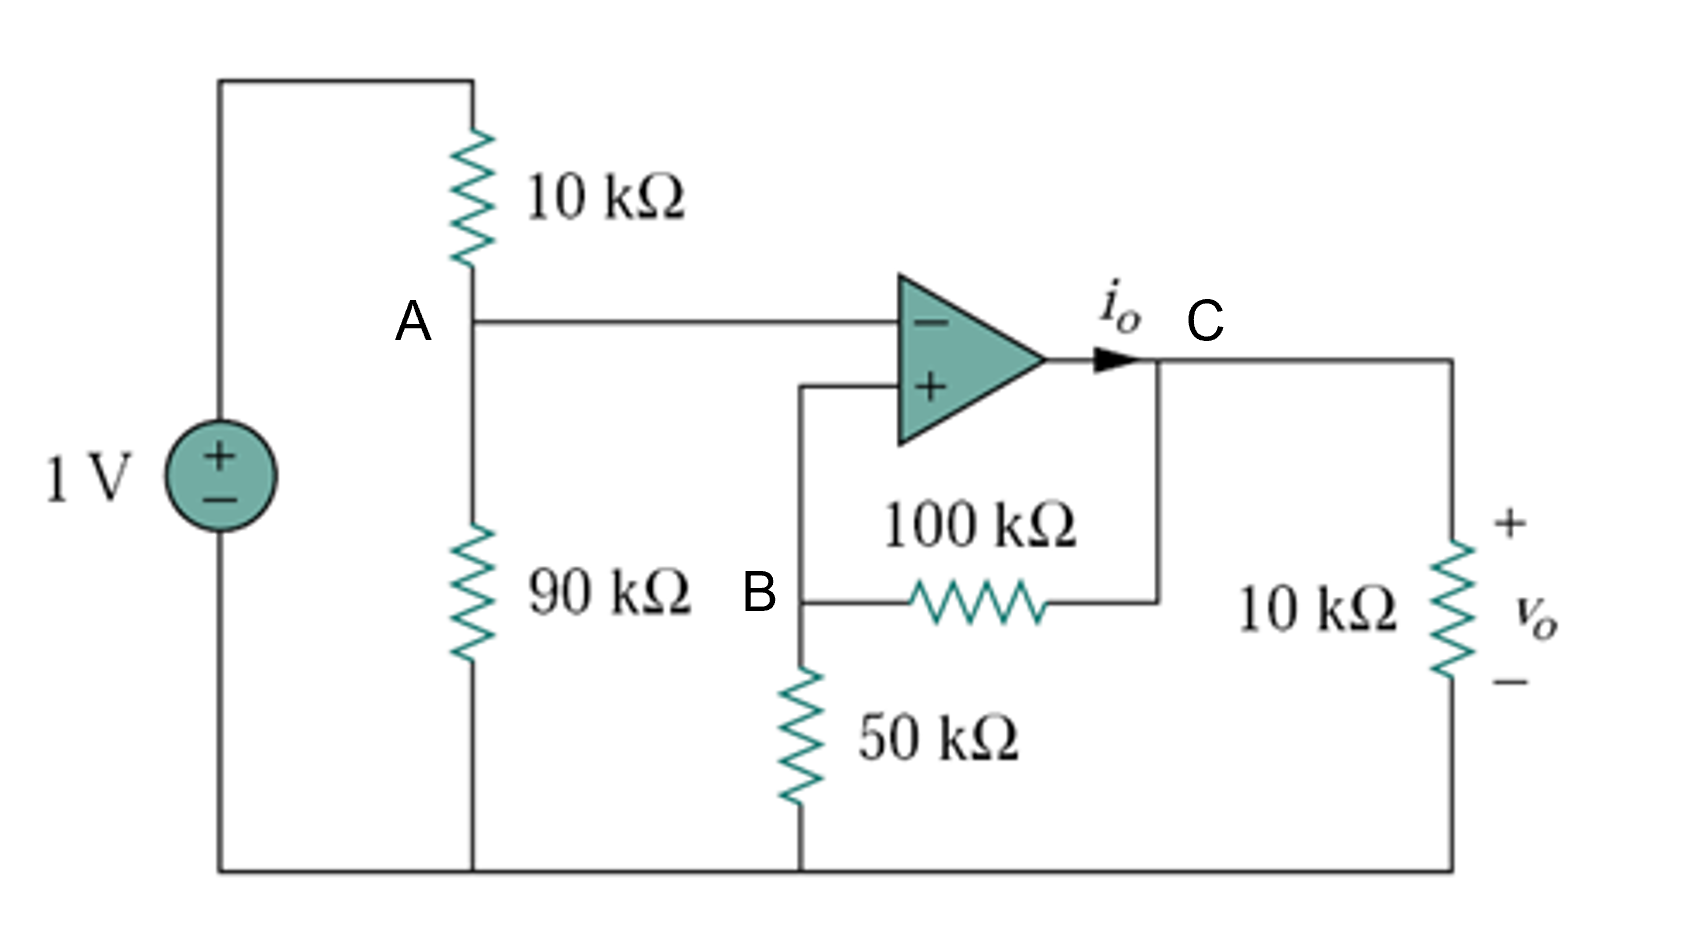
\includegraphics[width=0.7\textwidth]{pictures/topic4_b.png}
            \caption{Đề bài bài 4 hình thứ hai}
        \end{figure}
        \subsubsection{Tính giá trị $V_{out}$}
            \hspace*{0.6cm}Giả sử KĐTT là lý tưởng, ta có $V_{+} = V_{-} = V$. \\
            \hspace*{0.6cm}Áp dụng định luật K1 đối với nút A, ta có: $\frac{1 - V_{-}}{10} = \frac{V_{-}}{90} \Rightarrow V = V_{-} = 0.9V$. \\
            \hspace*{0.6cm}Áp dụng định luật K1 đối với nút B, ta có: $\frac{V_{+}}{50} = \frac{V_{out} - V_{+}}{100} \Rightarrow V_{out} = 3\cdot V= 2.7V$ \\
            \hspace*{0.6cm}Áp dụng định luật K1 đối với nút C, ta có: $\frac{V_{+} - V_{out}}{100} + \frac{V_{out}}{10} = i_{o} \Rightarrow i_{o} = 0.252V$ \\
        \subsection{Mô phỏng bằng proteus}
            \begin{itemize}
                \item Sử dụng Proteus để mô phỏng mạch như đề bài
                \item Các linh kiện sử dụng: Opamp, Resistor, DC Source, Ground.
                \item Kết quả mô phỏng proteus.
                \begin{figure}[H]
                    \centering
                    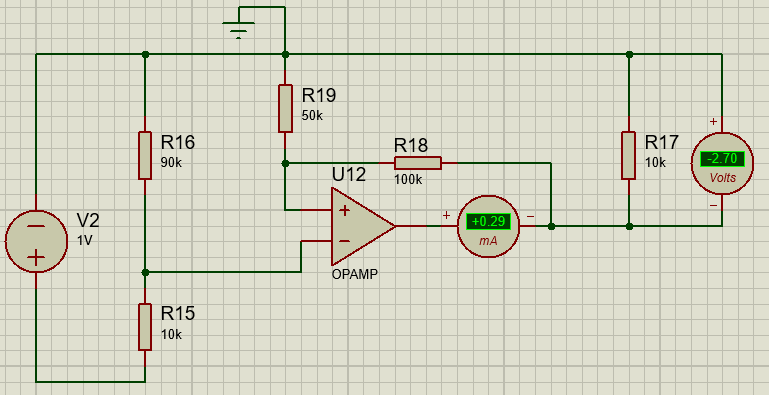
\includegraphics[width=0.7\textwidth]{pictures/result4_b.png}
                    \caption{Kết quả mô phỏng proteus bài 4 hình thứ hai}
                \end{figure}
            \end{itemize}
            \hspace*{0.6cm}Từ kết quả mô phỏng proteus, ta thấy giá trị $V_{out}$ của tải là 2.7V, giống với kết quả tính toán.

